%!TEX root = ../../controlbook.tex

%\begin{figure}[htb]
%  % Requires \usepackage{graphicx}
%  \centering
%  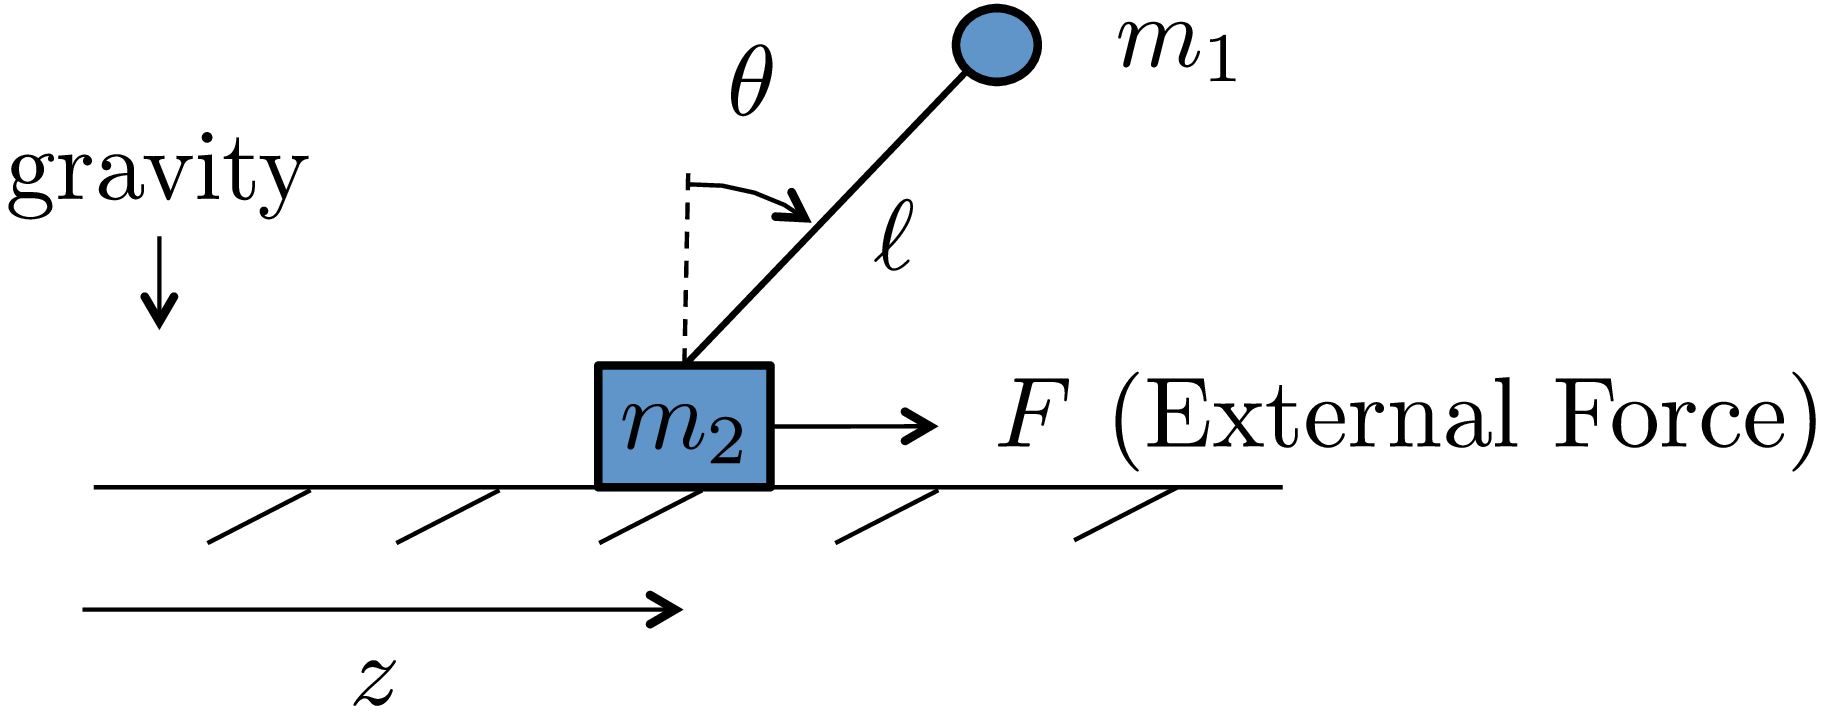
\includegraphics[width=0.6\textwidth]{6_design_studies/figures/hw_pendulum_defn.pdf}
%  \caption{Pendulum on a cart.}
%  \label{fig:int_pendulum_defn}
%\end{figure}

%\begin{figure}[tb!]
%\figureboxscale{0.5}{6_design_studies/figures/hw_pendulum_defn}
%{Pendulum on a cart.\label{fig:int_pendulum_defn}}
%\end{figure}

\begin{wrapfigure}{r}{0.5\textwidth}
  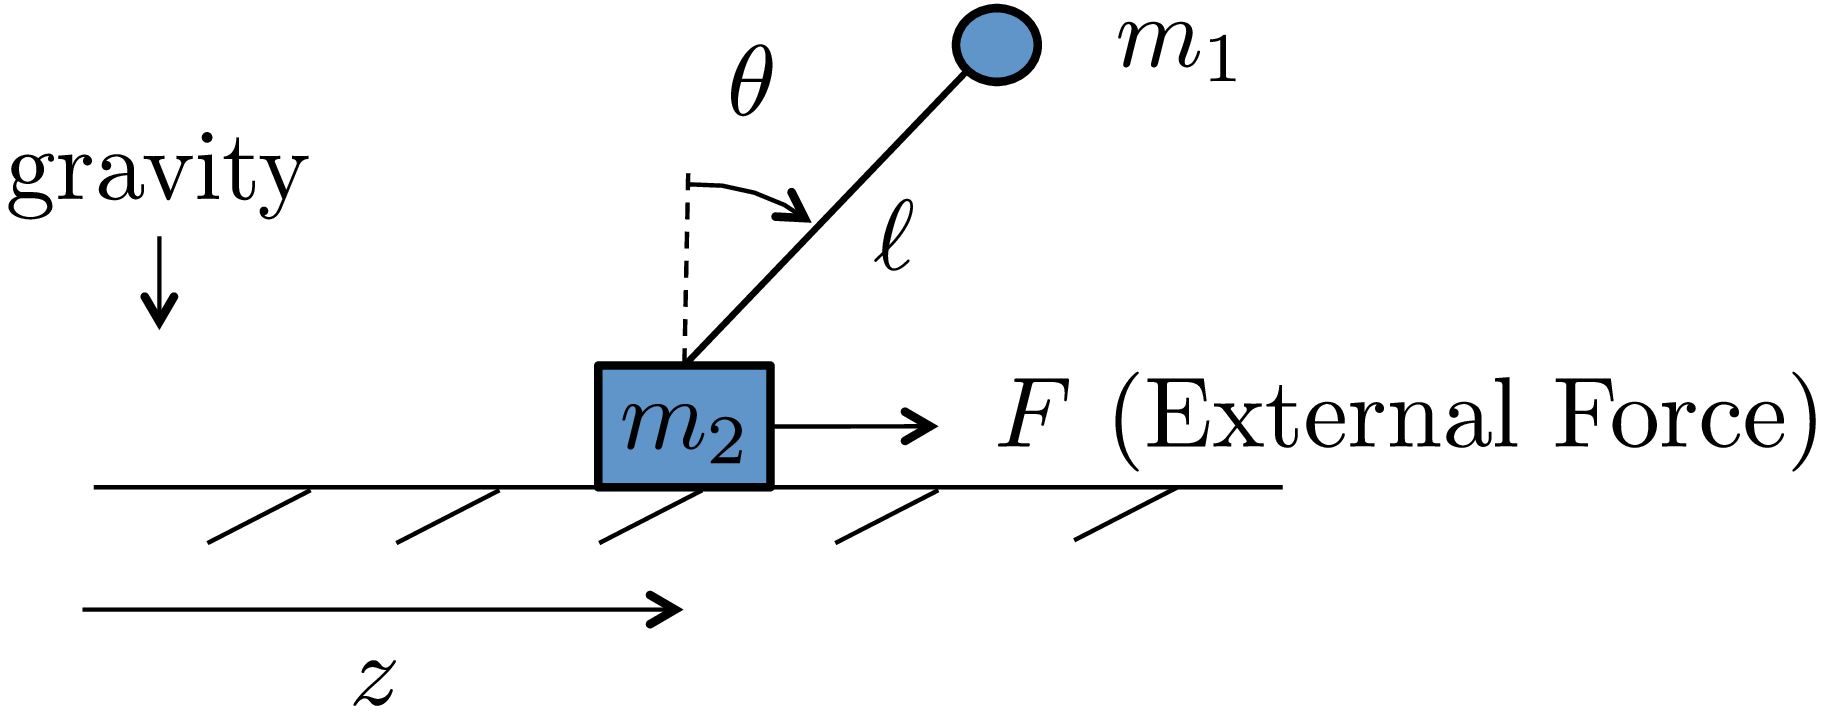
\includegraphics[width=0.49\textwidth]{6_design_studies/figures/hw_pendulum_defn.pdf}\\
  \caption{Pendulum on a cart.}
  \label{fig:int_pendulum_defn}
\end{wrapfigure}

Figure~\ref{fig:int_pendulum_defn} shows the pendulum on a cart system.  The position of the cart measured from the origin is $z$ and the linear speed of the cart is $\dot{z}$.  The angle of the pendulum from straight up is given by $\theta$, and the angular velocity is $\dot{\theta}$.  The rod is of length $\ell$, and has mass $m_1$, and is approximated as being infinitely thin. The cart has mass $m_2$.  Gravity acts in the down direction.  The only applied force is $F$, which acts in the direction of $z$.  The cart slides on a frictionless surface, but air friction produces a damping force equal to $-b\dot{z}$.

The physical constants are $m_1=0.25$~kg, $m_2=1.0$~kg, $\ell=1.0$~m, $g=9.8$~m/s$^2$, $b=0.05$~Ns.  The force is limited by $\abs{F}\leq 5$~N.
